\documentclass[12pt]{article}
\usepackage[utf8]{inputenc}
\usepackage[francais]{babel}
\usepackage{graphicx}

\title{Génie des Logiciels et des Systèmes\\Projet -- Partie 2}
\author{Victor Drouin Viallard}
\date{\today}

\begin{document}

\maketitle
\newpage

\tableofcontents
\newpage

\section{Introduction}
Cette deuxième partie du projet prend place, dans le scénario du projet, à l'issue de l'acceptation par le client du dossier préliminaire. On y est conduit à utiliser les outils de modélisation d'Eclipse pour répondre aux besoins du client.

\section{Structure du méta-modèle}
\subsection{Méta-modèle ECORE}
\paragraph{Analyse des besoins}
Le méta-modèle doit permettre de représenter un ensemble d'activités. L'utilisateur lit cet ensemble d'activités dans un sens donné et exécute chacunes d'elles en ayant par moments à choisir entre deux sous-ensembles d'activités ou à exécuter deux sous-ensembles d'activités en parallèle.

\paragraph{Description du méta-modèle}
Pour répondre aux besoins du commenditaire, j'ai donc décidé de définir la classe $Schedule$ pour représenter un ensemble de composants (class $Component$). J'ai alors défini la classe $Activity$ comme héritant de la class $Component$ de façon à pouvoir placer des activités dans cet ensemble. De plus j'ai défini la classe $Divergence$ (qui hérite aussi de la classe $Component$) de façon à représenter dans ce même ensemble les zones du scénario où l'utilisateur doit choisir entre plusieurs sous-ensembles ou les exécuter en parallèle. Un élément de type divergence possède donc un type pour distinguer les choix des exécutions en parallèle, ainsi qu'un ensemble de $Schedule$ en guise de sous-ensembles.
Ensuite j'ai pris soin de rajouter à $Activity$ une référence facultative vers un $Schedule$ de façon à pouvoir décrire des activités complexes en leur associant un sous-ensemble d'activités.
Enfin j'ai défini la classe $Scenario$ pour représenter le scénario dans son ensemble. Elle contient un lien vers le $Schedule$ principal et un nom pour décrire l'intitulé du scénario.

\paragraph{Tentatives avortées}
À plusieurs reprises mon méta-modèle a dû être modifié, notamment pour palier à ma méconaissance des langages OCL et Xtext. En effet, lors de l'utilisation de Sirius dans un premier temps, j'avais beaucoup de mal à imaginer qu'il soit possible de "relier" deux éléments consécutifs seulement à l'aide d'un tableau (celui contenu dans le $Schedule$). J'ai donc décidé d'ajouter une référence dans chaque $Component$ vers le $Component$ suivant et celui précédent. Le soucis est que cela rajoutait une redondance d'informations non nécessaire dans mon méta-modèle et que cela compliquait grandement l'écriture de modèles à l'aide de la syntaxe textuelle. Après une lecture plus attentive de la documentation OCL j'ai finalement réussi à trouver une façon de référencer l'élément suivant/précédent dans un $Schedule$ sans avoir recours à une référence explicite mais en utilisant l'index de l'élément courant dans le conteneur du $Schedule$. Il a donc en outre fallu que je mette dans mes classes $Component$ et $Schedule$ une référence vers l'élément parent de façon à pouvoir effectuer de pareille opérations (et cela à un sens concret pour le méta-modèle donc ce n'est pas abhérent), pour finalement aboutir au méta-modèle de la figure~\ref{Ecore}.

\begin{figure}
	\begin{center}
		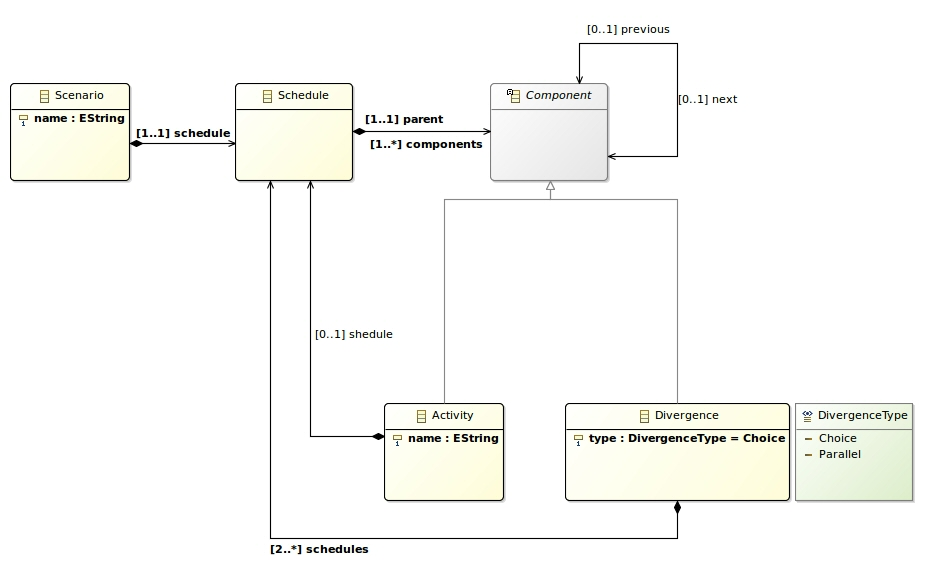
\includegraphics[width=\textwidth]{figures/scenario.png}
		\caption{Méta-modèle Ecore}
		\label{Ecore}
	\end{center}
\end{figure}

\subsection{Contraintes OCL}
\paragraph{Peu de contraintes nécessaires}
Compte tenu de la structure du méta-modèle que j'ai finalement adoptée, peu de contraintes OCL ont été nécessaire de façon à "vérouiller" mon méta-modèle. Les seules qui ont été nécessaires sont :
\begin{itemize}
	\item Noms interdits : pour interdire aux activités de porter certains noms qui peuvent porter à confusion, comme un nom vide ou "Activité".
	\item Noms uniques : pour interdire à deux activités d'un même ensemble ($Schedule$) de porter le même nom.
\end{itemize}
La deuxième contrainte est à la fois utile (et proposée par le sujet) et idiote. D'une part elle permet de référencer les activités par leur nom au sein d'un même $Schedule$ (ce qui peut être utile en Xtext), mais d'autre part il n'existe rien formellement qui interdise à un utilisateur de "Jouer aux échecs" deux fois dans la même journée. C'est donc une contrainte qui semble surtout avoir été suggéré par le sujet pour évaluer notre abilité à manipuler des contraintes OCL. Le sujet nous poussait en outre à jeter un oeil à l'opération $closure$ ce que j'aurai pu faire si il avait fallu garantir l'unicité du nom des activités au sein d'un scénario entier, mais il était bien écrit "au sein d'un même groupement" donc cela n'a pas été utile.

\paragraph{Contraintes avortées}
Toujours dans l'optiques où mon méta-modèle a évolué au fil de la réalisation du projet - car je ne connaissais pas assez bien OCL - j'avais aussi créé d'autres contraintes OCL dans une version antérieur, notamment pour garentir que deux $Component$ reliés par un lien suivant/précédent était dans le même $Schedule$, ou encore pour garantir qu'au sein d'un même $Schedule$ il existait un et un seul $Component$ n'ayant pas de suivant, et un et un seul $Component$ n'ayant pas de précédent. L'omission des liens suivant/précédent a rendu ces contraintes inutiles, puisque désormais l'unicité d'un "premier" et d'un "dernier" $Component$ au sein d'un même groupement est garantie par la structure ordonnée de la collection contenue dans $Schedule$. De la même façon c'est l'appartenance à cette collection qui garanti l'unicité du context des $Component$ successifs.

\section{Syntaxes concrètes}
\subsection{Syntaxe graphique avec Sirius}
\paragraph{Affichage des éléments de type $Divergence$}
Bien que la procédure ait été similaire à celle réalisée en TP, la création d'une syntaxe graphique avec Sirius a nécessité l'emploi de méthode quelques peu nouvelles (pour moi) et certaines fois cela m'a permi de mieux comprendre ce que à quoi servait "réellement" Sirius. Petit point délicat : la représentation des éléments de type $Divergence$. Tout d'abord il a fallu créer deux éléments graphiques pour chaque instance de $Divergence$ puisque la syntaxe graphique nécessitait un "cercle d'entrée" et d'un "cercle de sortie". Ensuite il fallait placer une croix dans les cercles représentant les entrées de "groupements au choix" et deux barres parallèles dans ceux représentant les entrées de "groupements parallèles" : j'ai pour cela cherché un méthode graphique avant de me rabattre sur l'utilisation du champ label, pour lequel j'ai du comprendre le fonctionnement d'OCL dans Sirius afin de distinguer chaque $Divergence$ selon son type pour alors afficher le texte "X" ou "//" en adéquation.

\paragraph{Des éléments $Edge$ complexes}
La plus grosse difficulté dans cette partie a été la création des éléments $Edge$ reliant les différents éléments $Component$ entre eux. En effet comme je l'ai dit plus haut, j'avais précédement esquivé (en partie) le problème en créant des références vers les éléments $Compoment$ suivant et précédent mais dès lors que je les avais retiré il me fallait utiliser correctement l'OCL pour retrouver autrement ces éléments. A l'aide des méthodes $collect$, $select$, $indexOf$ ou $at$ j'ai finalement réussi à faire ce que je voulais de façon à créer une syntaxe graphique très proche de celle suggérée par le client. On peut en voir un exemple sur la figure~\ref{Sirius}.

\begin{figure}
	\begin{center}
		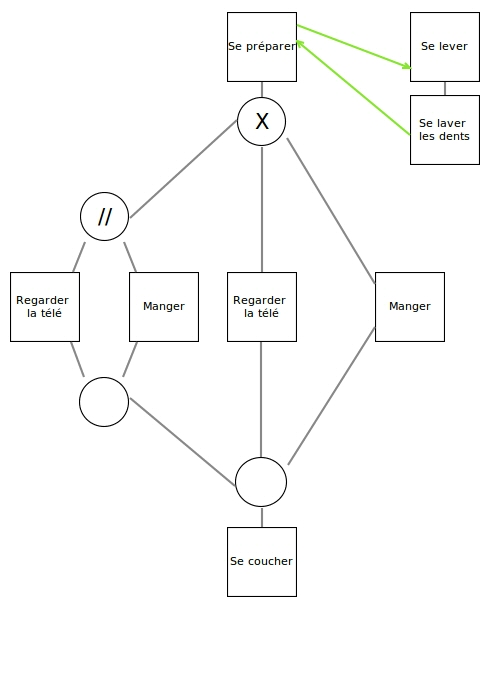
\includegraphics[width=\textwidth]{figures/sirius.png}
		\caption{Exemple de syntaxe graphique avec Sirius}
		\label{Sirius}
	\end{center}
\end{figure}

\subsection{Syntaxe textuelle avec Xtext}
\paragraph{Des changements dans le méta-modèle}
Comme je l'ai maintenant expliqué plusieurs fois, j'ai dû changer mon méta-modèle à la suite de problèmes rencontrés avec l'utilisation d'Xtext. En effet c'est à la suite de problèmes avec la création des références suivant/précédent que j'ai opté pour leur suppression, changeant par la suite mon méta modèle.

\paragraph{Une syntaxe concise}
J'ai commencé comme tous par utiliser la syntaxe créée automatiquement par Eclipse à partir de mon méta-modèle. Cependant cette syntaxe s'avère particulièrement lourde notamment par son utilisation systématiques d'accolades pour séparer les éléments. J'ai donc complètement édité cette syntaxe pour en créer une qui soit la plus simple et la plus compréhensible possible. On peut voir un exemple de modèle ainsi décrit sur la figure~\ref{Xtext}.

\begin{figure}
	\begin{center}
		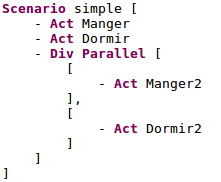
\includegraphics[]{figures/xtext.png}
		\caption{Exemple de syntaxe textuelle avec Xtext}
		\label{Xtext}
	\end{center}
\end{figure}


\section{Export HTML et requêtes EMF}
\subsection{Exportateur HTML en Acceleo}
Sur cette partie j'ai pris soin de découper au mieux mon code afin de le rendre le plus modulaire possible, tout en respectant avec attention la structure HTML de façon à rendre un fichier HTML valide vis-à-vis des spécifications de W3C. Je n'ai pas porté attention au CSS puisque l'affichage standard était suffisamment clair.

\subsection{Requêtes EMF}
Au jour de rendu du rapport je n'ai pas encore pris le temps d'effectuer cette partie.

\section{Conclusion}
Je suis globalement satisfait du travail effectué, bien que n'ayant pas fait les requêtes EMF. Le projet m'a permis de réellement mieux comprendre le fonctionnement des outils de modélisation d'Eclipse qui me paraissaient assez obscures jusqu'alors, et je suis agréablement surpris de m'appercevoir que cette fois ci je n'ai eu aucun problème avec mes workspaces Eclipse ce qui m'a permis d'avancer sereinement dans le projet.
Je regrète néanmoinsl l'utilisation de ce logiciel car, même si il concentre un grand nombre plugins utiles, son interface est souvent peu intuitive et il est par exemple souvent délicat pour le néophyte de comprendre comment il effectue la gestion des workspace et des projets ce qui conduit bien souvent à des erreurs de manipulations fatales. Je pense en outre que nous aurions bien plus rapidement compris le fonctionnement de ces technologies, de façon à réellement les maîtriser et donc pouvoir les réutiliser, si nous avions eu à les manipuler "à la main" (sans utiliser un clicodrôme lourd et complexe).

\end{document}